\documentclass[12pt,titlepage]{article}
\usepackage[margin=1.25in]{geometry}
\usepackage{graphicx,amsmath,blindtext}

%% Variables definition
\newcommand{\vSubject}{Matematika 3}
\newcommand{\vSubtitle}{Euclidian Distance}
\newcommand{\vName}{Dicha Zelianivan Arkana}
\newcommand{\vNIM}{2241720002}
\newcommand{\vClass}{1i}
\newcommand{\vDepartment}{Information Technology}
\newcommand{\vStudyProgram}{D4 Informatics Engineering}

%% [START] Tikz related stuff
\usepackage{tikz}
\usetikzlibrary{svg.path,calc,shapes.geometric,shapes.misc}
\tikzstyle{terminator} = [rectangle, draw, text centered, rounded corners = 1em, minimum height=2em]
\tikzstyle{preparation} = [chamfered rectangle, chamfered rectangle sep=0.75em, draw, text centered, minimum height = 2em]
\tikzstyle{process} = [rectangle, draw, text centered, minimum height=2em]
\tikzstyle{decision} = [diamond, aspect=2, draw, text centered, minimum height=2em]
\tikzstyle{data}=[trapezium, draw, text centered, trapezium left angle=60, trapezium right angle=120, minimum height=2em]
\tikzstyle{connector} = [line width=0.25mm,->]
%% [END] Tikz related stuff

%% [START] Fancy header related stuff
\usepackage{fancyhdr}
\pagestyle{fancy}
\setlength{\headheight}{15pt} % compensate fancyhdr style
\fancyhead{}
\fancyfoot{}
\fancyfoot[L]{\thepage}
\fancyfoot[R]{\textit{\vSubject - \vSubtitle}}
\renewcommand{\footrulewidth}{0.4pt}% default is 0pt, overline for footer
%% [END] Fancy header related stuff

%% [START] Custom tabular command related stuff
\usepackage{tabularx}
\newcommand{\details}[2]{
    #1 & #2  \\
}
%% [END] Custom tabular command related stuff

%% [START] Figure related stuff
\newcommand{\image}[3][1]{
    \begin{figure}[h]
        \centering
        \includegraphics[#1]{#2}
        \caption{#3}
        \label{#3}
    \end{figure}
}
%% [END] Figure related stuff

\begin{document}
\begin{titlepage}
    \centering
    \vfill
    {\bfseries\LARGE
        \vSubject\\
        \vskip0.25cm
        \vSubtitle
    }
    \vfill
    \includegraphics[width=6cm]{images/polinema-logo.png}
    \vfill
    {
        \textbf{Name}\\
        \vName\\
        \vskip0.5cm
        \textbf{NIM}\\
        \vNIM\\
        \vskip0.5cm
        \textbf{Class}\\
        \vClass\\
        \vskip0.5cm
        \textbf{Department}\\
        \vDepartment\\
        \vskip0.5cm
        \textbf{Study Program}\\
        \vStudyProgram
    }
\end{titlepage}

\tableofcontents
\pagebreak

\section{Euclidian Distance}
\subsection{Task 1}
\begin{enumerate}
    \item {
        $(2, 4)~\&~(3, 6)$
        \begin{align*}
            (2, 4)~\&~(3, 6) &= \sqrt{(3 - 2)^2 + (6 - 4)^2} \\
            &= \sqrt{1 + 4} \\
            &= \sqrt{5} \\
            &= 2.23
        \end{align*}
    }
    \item {
        $(2, 4)~\&~(5, 3)$
        \begin{align*}
            (2, 4)~\&~(5, 3) &= \sqrt{(5 - 2)^2 + (3 - 4)^2} \\
            &= \sqrt{9 + 1} \\
            &= \sqrt{10} \\
            &= 3.16
        \end{align*}
    }
    \item {
        $(2, 4)~\&~(7, 1)$
        \begin{align*}
            (2, 4)~\&~(7, 1) &= \sqrt{(7 - 2)^2 + (1 - 4)^2} \\
            &= \sqrt{25 + 9} \\
            &= \sqrt{34} \\
            &= 5.83
        \end{align*}
    }
    \item {
        $(2, 4)~\&~(6, 8)$
        \begin{align*}
            (2, 4)~\&~(6, 8) &= \sqrt{(6 - 2)^2 + (8 - 4)^2} \\
            &= \sqrt{16 + 16} \\
            &= \sqrt{32} \\
            &= 5.65
        \end{align*}
    }
    % cartesian representation
    \begin{center}
        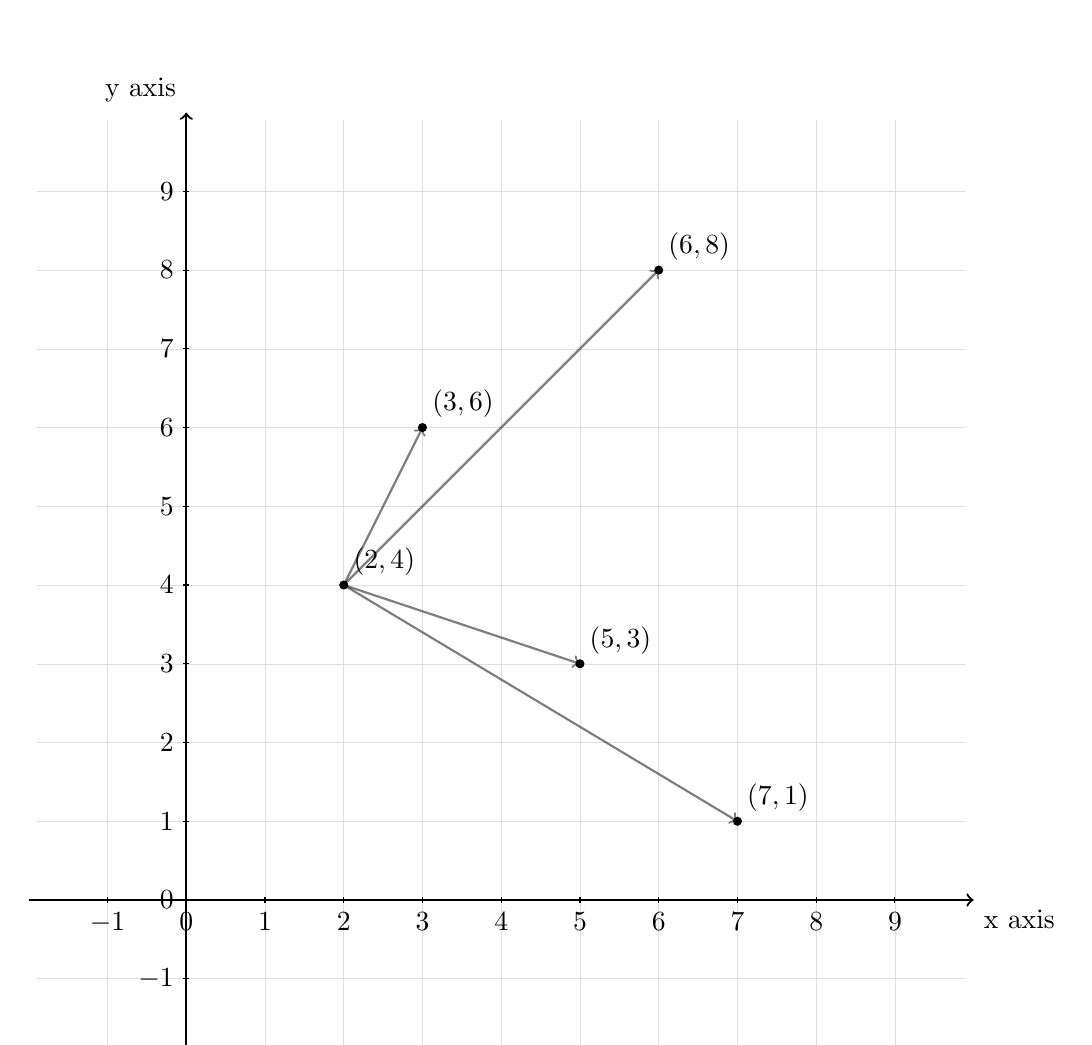
\begin{tikzpicture}
            \draw[step=1cm,gray,very thin,opacity=0.25] (-1.9,-1.9) grid (9.9,9.9);
            \draw[thick,->] (-2,0) -- (10,0) node[anchor=north west] {x axis};
            \draw[thick,->] (0,-2) -- (0,10) node[anchor=south east] {y axis};
            \foreach \x in {-1,0,1,2,3,4,5,6,7,8,9}
                \draw (\x cm,1pt) -- (\x cm,-1pt) node[anchor=north] {$\x$};
            \foreach \y in {-1,0,1,2,3,4,5,6,7,8,9}
                \draw (1pt,\y cm) -- (-1pt,\y cm) node[anchor=east] {$\y$};
            \draw[fill=black] (2,4) circle (0.05cm) node[anchor=south west] {$(2, 4)$};
            \draw[fill=black] (3,6) circle (0.05cm) node[anchor=south west] {$(3, 6)$};
            \draw[fill=black] (5,3) circle (0.05cm) node[anchor=south west] {$(5, 3)$};
            \draw[fill=black] (7,1) circle (0.05cm) node[anchor=south west] {$(7, 1)$};
            \draw[fill=black] (6,8) circle (0.05cm) node[anchor=south west] {$(6, 8)$};
            \draw[thick,->,opacity=0.5] (2,4) -- (3,6);
            \draw[thick,->,opacity=0.5] (2,4) -- (5,3);
            \draw[thick,->,opacity=0.5] (2,4) -- (7,1);
            \draw[thick,->,opacity=0.5] (2,4) -- (6,8);
        \end{tikzpicture}
    \end{center}
\end{enumerate}

\subsection{Task 2}
\begin{figure}[h]
    \centering
    \includegraphics[width=0.8\textwidth]{./images/task-2.png}
\end{figure}

\subsection{Additional Task}
\begin{enumerate}
    \item {
        $(-1, 2)~\&~(3, 5)$
        \begin{align*}
            (2, 3)~\&~(4, 1) &= \sqrt{(4 - 2)^2 + (1 - 3)^2} \\
            &= \sqrt{4 + 4} \\
            &= \sqrt{8} \\
            &= 2.82
        \end{align*}
        % cartesian representation, at the center
        \begin{center}
            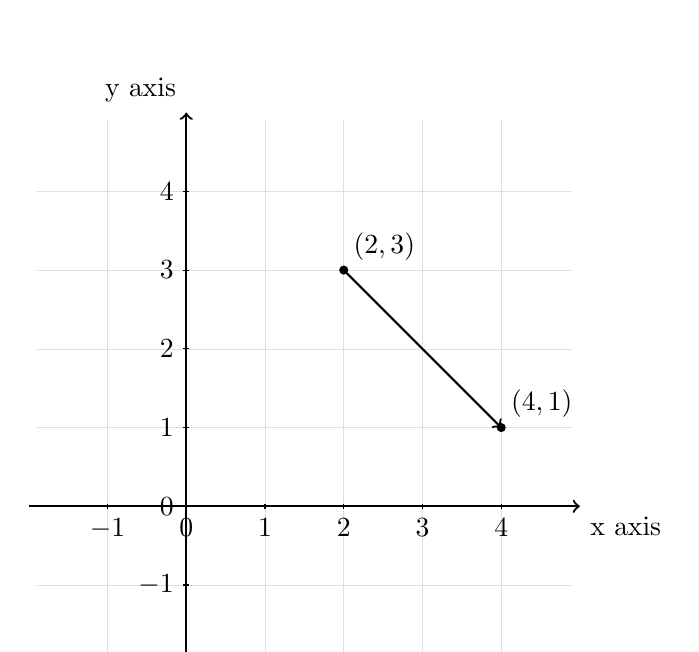
\begin{tikzpicture}
                \draw[step=1cm,gray,very thin,opacity=0.25] (-1.9,-1.9) grid (4.9,4.9);
                \draw[thick,->] (-2,0) -- (5,0) node[anchor=north west] {x axis};
                \draw[thick,->] (0,-2) -- (0,5) node[anchor=south east] {y axis};
                \foreach \x in {-1,0,1,2,3,4}
                    \draw (\x cm,1pt) -- (\x cm,-1pt) node[anchor=north] {$\x$};
                \foreach \y in {-1,0,1,2,3,4}
                    \draw (1pt,\y cm) -- (-1pt,\y cm) node[anchor=east] {$\y$};
                \draw[fill=black] (2,3) circle (0.05cm) node[anchor=south west] {$(2, 3)$};
                \draw[fill=black] (4,1) circle (0.05cm) node[anchor=south west] {$(4, 1)$};
                \draw[thick,->] (2,3) -- (4,1);
            \end{tikzpicture}
        \end{center}
    }
    \pagebreak
    \item {
        $(6, 2)~\&~(9, 7)$
        \begin{align*}
            (6, 2)~\&~(9, 7) &= \sqrt{(9 - 6)^2 + (7 - 2)^2} \\
            &= \sqrt{9 + 25} \\
            &= \sqrt{34} \\
            &= 5.83
        \end{align*}
        % cartesian representation, at the center
        \begin{center}
            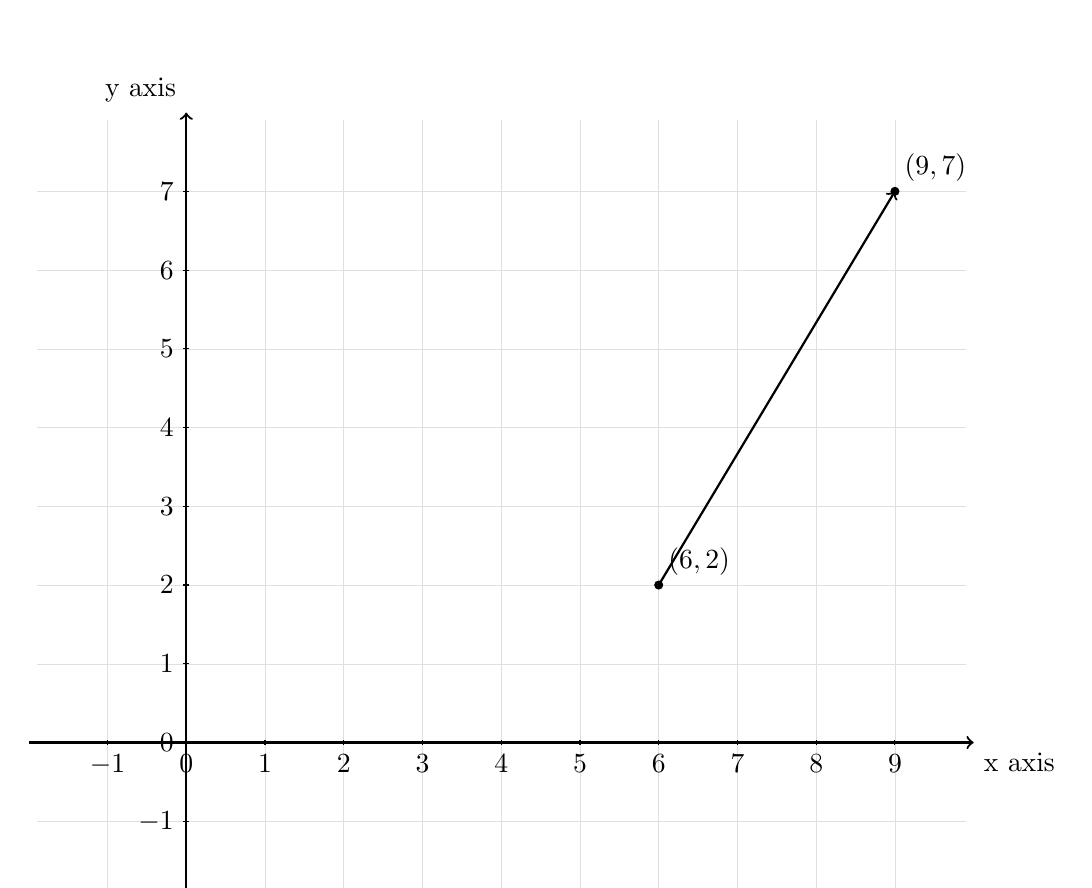
\begin{tikzpicture}
                \draw[step=1cm,gray,very thin,opacity=0.25] (-1.9,-1.9) grid (9.9,7.9);
                \draw[thick,->] (-2,0) -- (10,0) node[anchor=north west] {x axis};
                \draw[thick,->] (0,-2) -- (0,8) node[anchor=south east] {y axis};
                \foreach \x in {-1,0,1,2,3,4,5,6,7,8,9}
                    \draw (\x cm,1pt) -- (\x cm,-1pt) node[anchor=north] {$\x$};
                \foreach \y in {-1,0,1,2,3,4,5,6,7}
                    \draw (1pt,\y cm) -- (-1pt,\y cm) node[anchor=east] {$\y$};
                \draw[fill=black] (6,2) circle (0.05cm) node[anchor=south west] {$(6, 2)$};
                \draw[fill=black] (9,7) circle (0.05cm) node[anchor=south west] {$(9, 7)$};
                \draw[thick,->] (6,2) -- (9,7);
            \end{tikzpicture}
        \end{center}
    }
    \pagebreak
    \item {
        $(3, 4)~\&~(6, 5)$
        \begin{align*}
            (3, 4)~\&~(6, 5) &= \sqrt{(6 - 3)^2 + (5 - 4)^2} \\
            &= \sqrt{9 + 1} \\
            &= \sqrt{10} \\
            &= 3.16
        \end{align*}
        % cartesian representation, at the center
        \begin{center}
            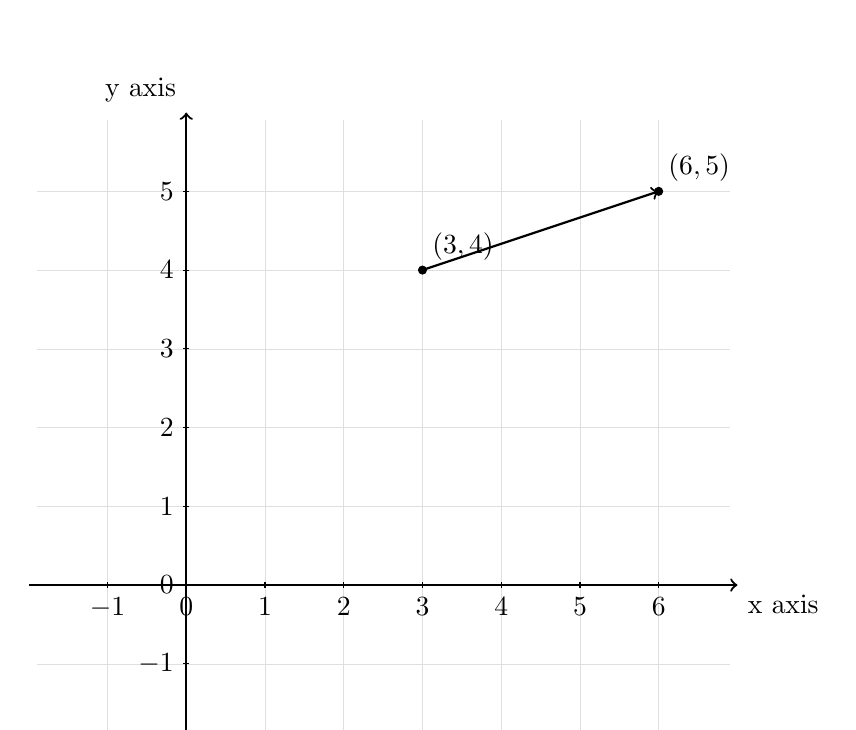
\begin{tikzpicture}
                \draw[step=1cm,gray,very thin,opacity=0.25] (-1.9,-1.9) grid (6.9,5.9);
                \draw[thick,->] (-2,0) -- (7,0) node[anchor=north west] {x axis};
                \draw[thick,->] (0,-2) -- (0,6) node[anchor=south east] {y axis};
                \foreach \x in {-1,0,1,2,3,4,5,6}
                    \draw (\x cm,1pt) -- (\x cm,-1pt) node[anchor=north] {$\x$};
                \foreach \y in {-1,0,1,2,3,4,5}
                    \draw (1pt,\y cm) -- (-1pt,\y cm) node[anchor=east] {$\y$};
                \draw[fill=black] (3,4) circle (0.05cm) node[anchor=south west] {$(3, 4)$};
                \draw[fill=black] (6,5) circle (0.05cm) node[anchor=south west] {$(6, 5)$};
                \draw[thick,->] (3,4) -- (6,5);
            \end{tikzpicture}
        \end{center}
    }
\end{enumerate}

\pagebreak

\section{Cityblock Distance}
\subsection{Task 3}
\begin{enumerate}
    \item {
        $(2, 4)~\&~(3, 6)$
        \begin{align*}
            (2, 4)~\&~(3, 6) &= |3-2| + |6-4| \\
            &= 1 + 2 \\
            &= 3
        \end{align*}
    }
    \item {
        $(2, 4)~\&~(5, 3)$
        \begin{align*}
            (2, 4)~\&~(5, 3) &= |5-2| + |3-4| \\
            &= 3 + 1 \\
            &= 4
        \end{align*}
    }
    \item {
        $(2, 4)~\&~(7, 1)$
        \begin{align*}
            (2, 4)~\&~(7, 1) &= |7-2| + |1-4| \\
            &= 5 + 3 \\
            &= 8
        \end{align*}
    }
    \item {
        $(2, 4)~\&~(6, 8)$
        \begin{align*}
            (2, 4)~\&~(6, 8) &= |6-2| + |8-4| \\
            &= 4 + 4 \\
            &= 8
        \end{align*}
    }
    % cartesian representation
    \pagebreak
    \begin{center}
        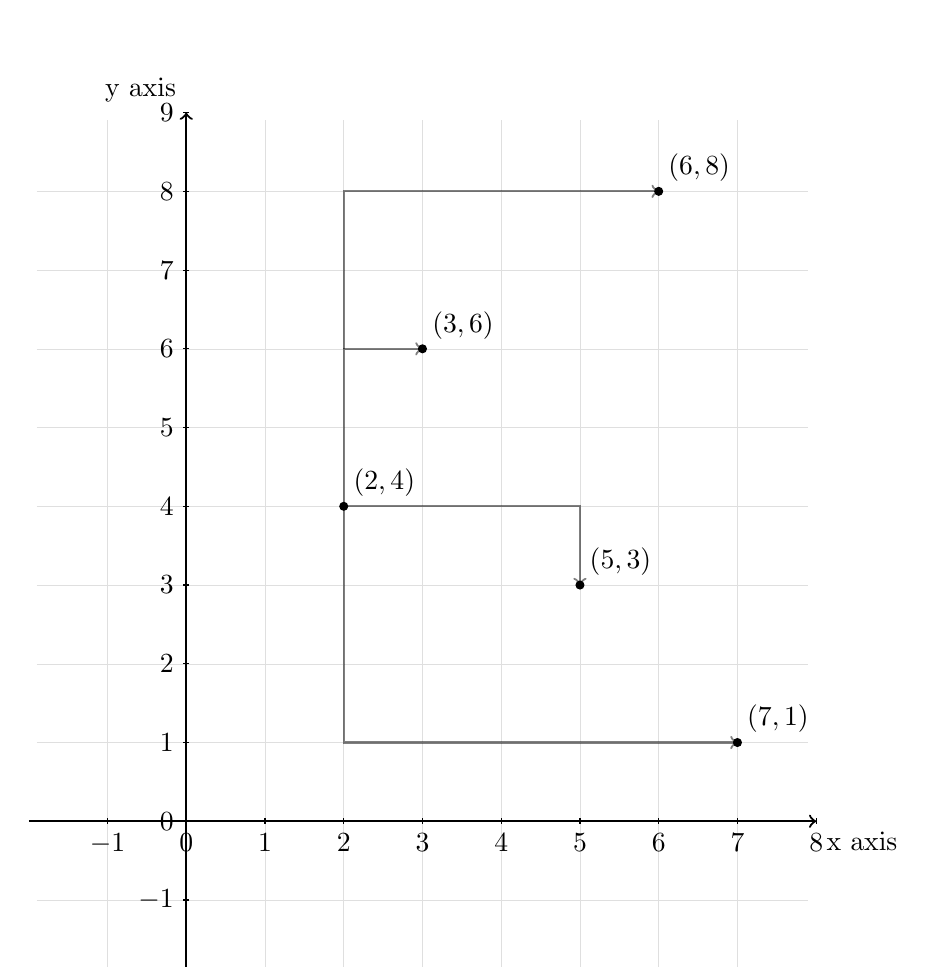
\begin{tikzpicture}
            \draw[step=1cm,gray,very thin,opacity=0.25] (-1.9,-1.9) grid (7.9,8.9);
            \draw[thick,->] (-2,0) -- (8,0) node[anchor=north west] {x axis};
            \draw[thick,->] (0,-2) -- (0,9) node[anchor=south east] {y axis};
            \foreach \x in {-1,0,1,2,3,4,5,6,7,8}
                \draw (\x cm,1pt) -- (\x cm,-1pt) node[anchor=north] {$\x$};
            \foreach \y in {-1,0,1,2,3,4,5,6,7,8,9}
                \draw (1pt,\y cm) -- (-1pt,\y cm) node[anchor=east] {$\y$};
            \draw[fill=black] (2,4) circle (0.05cm) node[anchor=south west] {$(2,4)$};
            \draw[fill=black] (5,3) circle (0.05cm) node[anchor=south west] {$(5,3)$};
            \draw[fill=black] (3,6) circle (0.05cm) node[anchor=south west] {$(3,6)$};
            \draw[fill=black] (7,1) circle (0.05cm) node[anchor=south west] {$(7,1)$};
            \draw[fill=black] (6,8) circle (0.05cm) node[anchor=south west] {$(6,8)$};
            \draw[thick,->,opacity=0.5] (2,4) -- (2,6) -- (3,6);
            \draw[thick,->,opacity=0.5] (2,4) -- (5,4) -- (5,3);
            \draw[thick,->,opacity=0.5] (2,4) -- (2,1) -- (7,1);
            \draw[thick,->,opacity=0.5] (2,6) -- (2,8) -- (6,8);
        \end{tikzpicture}
    \end{center}
\end{enumerate}

\subsection{Task 4}
\begin{figure}[h]
    \centering
    \includegraphics[width=0.8\textwidth]{./images/task-4.png}
\end{figure}

\section{Conclusion}
\subsection{Task 5}
\begin{enumerate}
    \item {
        Euclidian distance is the distance between two points in a plane. The formula is:
        \begin{align*}
            d(p, q) = \sqrt{(q_1 - p_1)^2 + (q_2 - p_2)^2}
        \end{align*}
    }
    \item {
        Cityblock distance is the distance between two points in a plane, but the distance is calculated by the sum of the absolute differences of their Cartesian coordinates. The formula is:
        \begin{align*}
            d(p, q) = |q_1 - p_1| + |q_2 - p_2|
        \end{align*}
    }
\end{enumerate}
Both of them can be used to find a distance between two points, this can be applied in real life such as finding the shortest distance between two landmarks, clustering, and etc.

\end{document}

